\section{data}\label{sec:data}


\subsection{GLAM}



\subsection{ABACUS}



Fig. \ref{fig:data} shows the mean bispectrum (left) and the mean power spectrum (right) for the GLAM and ABACUS simulations, relative to the spectra without the BAO signal, which is simulation-based for the GLAM realizations and theory-based for the ABACUS.

\begin{figure*}
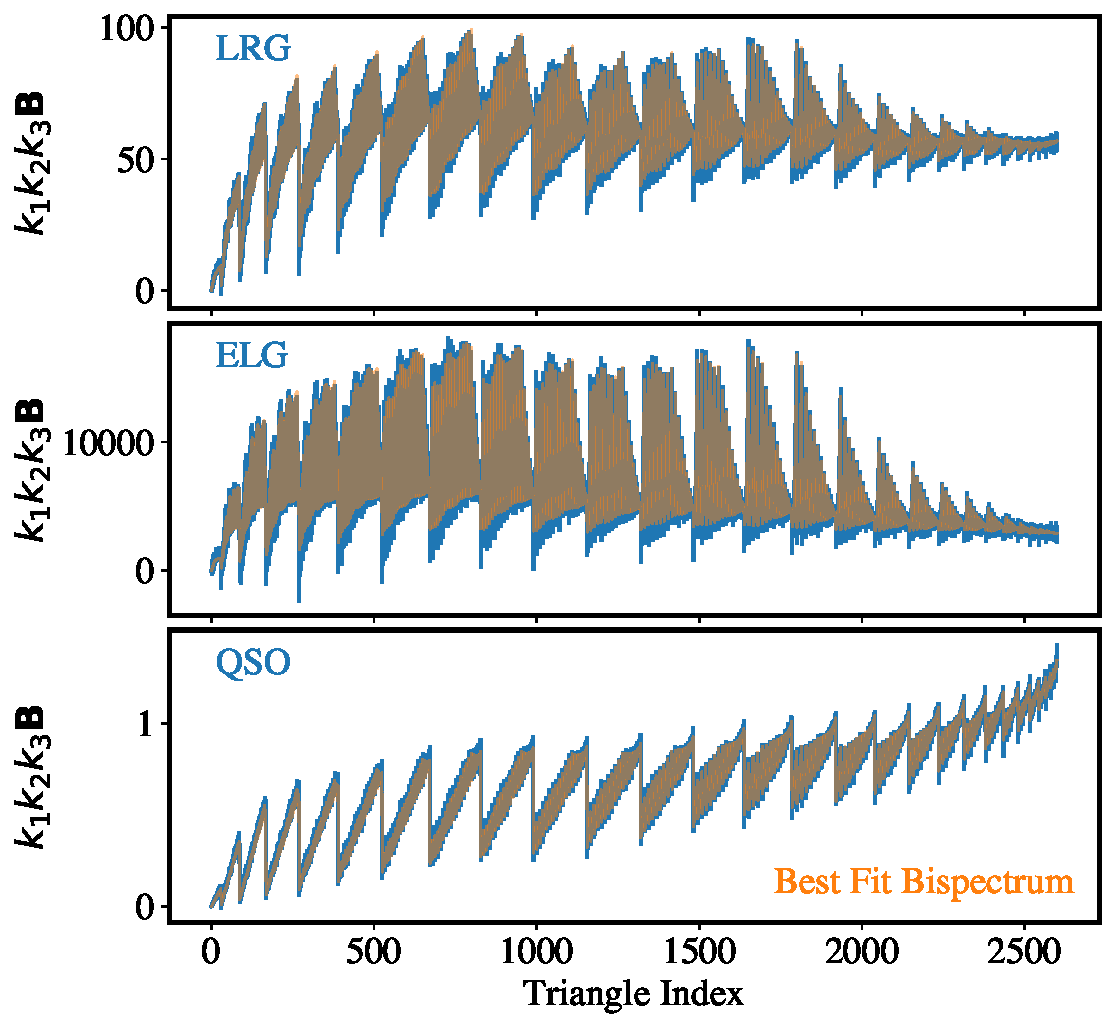
\includegraphics[width=\textwidth]{figures/spectra.pdf}
\caption{Spectra of ABACUS, GLAM, and MOLINO simulations. Top: Mean bispectrum and power spectrum of simulations relative to smooth spectrum either from the mocks (GLAM) or fitting formula (ABACUS). Bottom: Normalized dispersion of bispectrum and power spectrum.}\label{fig:data}
\end{figure*}
